\documentclass{article}
\usepackage{G7.32-2017}
\begin{document}


{\Huge
Ну--с, класс я написал. Посмотрим, что из этого выйдет...

}


\Executors

Здесь должны быть по--умолчанию список исполнителей, но мне набирать его оформление влом. Поэтому это просто заголовок

\Repherat

Генерируемый автоматически отчёт, наверное, не надо добавлять. Это пока что не в моих силах.

Пишем здесь что--то....

Еще пишем... и вообще, может быть, здесь надо написать какой--нибудь абзац и посмотреть, как \LaTeX отреагирует на это. Ну, например, это абзац  абзац абзац абзац абзац абзац абзац абзац абзац абзац абзац абзац абзац абзац абзац абзац абзац абзац абзац абзац абзац абзац

\newpage

\tableofcontents

\TermAndDefine

Здесь должны быть термины и определения, но по--ГОСТ'у их вроде по--особому описывать не надо, но это не точно.

\listAbbreviationAndNotation

Здесь тоже по--идее не надо чего--то сверхъестественного.

\Intoduction

Это введение. Здесь можно описать введение. Текст текст текст текст текст текст текст текст текст текст текст текст текст текст текст текст текст текст текст текст текст текст текст текст текст

\section{Первый заголовок секции в этом... нечто. Интересно, тут будут переносы? По ГОСТу нет}

Ну, короче, пишем здесь чего--нибудь, но, главное, чтобы не на всю страницу(Это для теста)

\section{Второй заголовок секции}

abcdef 

defjhi.....

\subsection{Заголовок подсекции. Допустим, с секцией всё хорошо...}

Попробуем таблицу(Таблица \ref{tablekey}).

\begin{table}[h!]
\caption{Заголовок нужен?}
	\begin{center}
		\begin{tabular}{|c|c|}
			\hline 
			1 & 2 \\ 
			\hline 
			3 & 4 \\ 
			\hline 
		\end{tabular} 
	\end{center}
\label{tablekey}
\end{table}

Попробуем графон(Рисунок \ref{fig:fortitle})

\begin{figure}[h!]
	\centering
	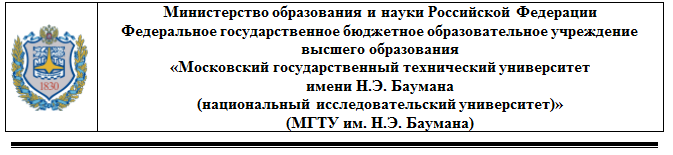
\includegraphics[width=0.7\linewidth]{For_title}
	\caption{Надпись под рисунком}
	\label{fig:fortitle}
\end{figure}

\section{Третья секция}

Попробуем списки:

\begin{GostItemize}
\item Надеюсь, с этим элементом всё по--ГОСТу. Хотя стандартный itemize и enumerare не совсем подходят под описание ГОСТа, поэтому пришлось определить свои окружения.

\item Хотя ничто не запрещает пользоваться переопределёнными itemize и enumerate, но выглядеть это будет не совсем так, как в ГОСТе
\end{GostItemize}

\begin{GostEnumerate}
\item Это нумерация через цифры. Конечно, пипец писать эту нумерацию. Хоть \LaTeX и не Python, если бы не несколько оговорок из книги Львовского и знание, что такое пространства имён, хрена с два я бы написал это окружение

\item Ну, вроде всё нумеруется нормально
\begin{GostEnumerate}
\item Можно попробовать уйти в нумерацию поглубже

\item Но нужно учесть, что...

\begin{GostEnumerate}
\item Глубина нумерации не больше 3.

\item Хотя, если понадобится глубже, просто скажите, я ещё добавлю счётчиков.
\end{GostEnumerate}
\end{GostEnumerate}
\end{GostEnumerate}

\begin{GostSymbolEnumerate}
\item Также есть символьная нумерация.

\item ГОСТ это допускает, так что я сделал это.
\end{GostSymbolEnumerate}

\Conclusion

Здесь должно быть заключение о степени заболевания того человека, который написал этот ГОСТ.

\ListSource

Здесь список использованных источников, так как ссылок нет, то оформлять через GostEnumerate, ну, или через обычный enumerate.

\Appendix

Вроде в аппендиксах ничего не ставится в заголовке кроме самого аппендикса, но если что --- скажите.

Попробуем графику(Рисунок \ref{fig:app})

\begin{figure}[h!]
	\centering
	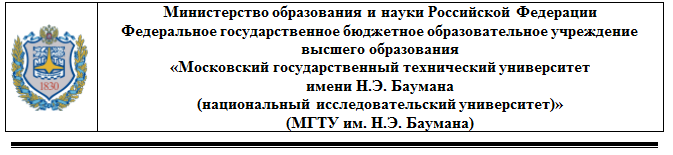
\includegraphics[width=0.7\linewidth]{For_title}
	\caption{1 графон}
	\label{fig:app}
\end{figure}

\begin{figure}[h!]
	\centering
	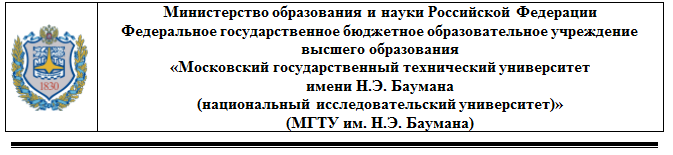
\includegraphics[width=0.7\linewidth]{For_title}
	\caption{2 графон}
	\label{fig:app2}
\end{figure}

\Appendix

Кстати, я не знаю, как насчёт всех букв в азбуке \LaTeX, так что дохренилиард аппендиксов добавлять не советую.

Попробуем таблицу(таблица \ref{tab:tab})

\begin{table}[h!]
	\caption{Заголовок???}
	\centering
	\begin{tabular}{|c|c|}
		\hline 
		1 & 2 \\ 
		\hline 
		3 & 4 \\ 
		\hline 
	\end{tabular}
\label{tab:tab}
\end{table}

\begin{figure}[h!]
	\centering
	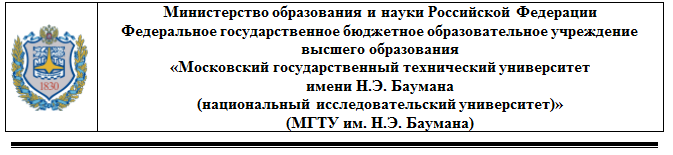
\includegraphics[width=0.7\linewidth]{For_title}
	\caption{Тестовая пикча}
	\label{fig:fortitle3}
\end{figure}

\Appendix


\Finish

\end{document}